\documentclass{article}
\usepackage[utf8]{inputenc}
\usepackage{biblatex}
\usepackage{graphicx}
\usepackage{subcaption}
\usepackage{amsmath}
\usepackage{upgreek}
\usepackage{amssymb}
\addbibresource{main.bib}

\setlength{\parskip}{1em}
\setlength{\parindent}{0em}
\title{Methods for particle tracking in zebrafish}
\author{Yngve Mardal Moe}
\date{November 2021}

\begin{document}

\maketitle

\section{Introduction}
This document describes the workflow for tracking particles in zebrafish embryo. The workflow is separated into three parts.

\begin{itemize}
    \item Preprocessing and particle tracking
    \item Estimating vasculature geometry
    \item Estimating velocities and pressures
\end{itemize}

We disregarded the results for all files where the vessel background image had different shape compared to the particle videos.

\section{Preprocessing and particle tracking}
Tracking particles is done using \texttt{trackpy}, a Python library for PTV. TrackPy uses the method described in \cite{crocker1996methods}, which roughly speaking does as follows:

\begin{enumerate}
    \item Preprocess each frame using a band-pass filter. This removes high-frequency noise and low-frequency sensor differences. The high-pass part of the band-pass filter is decided based on the particles' estimated size
    \item Find possible particles. This will find a large amount of false positives that needs to be filtered away.
    \item Filter away false positive particles. We require that particles are separated by at least 6 pixels and that the particles have total mass (i.e. total integrated brightness) $\geq 50$.
    \item Link particles between frames by searching the next frame in a 16 pixel radius around the particle's position in the current frame. Our settings allows particles to be present for only every second frame.
    \item Exclude particles that are not present in at least two frames.
\end{enumerate}

Step 1-3 are performed by the \texttt{trackpy.batch} function, step 4 is performed by the \texttt{trackpy.link} function and step 5 is performed by the \texttt{trackpy.filter\_stubs} function. We noticed, however, that this default preprocessing is insufficient. We therefore perform the following preprocessing instead

\begin{enumerate}
    \item For each pixel, compute its average value across each frames. This gives us a background-signal estimate
    \item For each pixel, subtract the background signal and set all negative pixels equal to 0
    \item Perform a morphological (greyscale) opening with a $3\times3$ structuring element
    \item Perform a morphological (greyscale) closing with a $5\times5$ structuring element
    \item Modify the dynamic range to be between 2 and 50 (clipping pixel values between 2 and 50)
    \item Transform each pixel value using the transform $T(x) = 255  (x - 2)/(50 - 2)$
\end{enumerate}

By disabling the default preprocessing in \texttt{trackpy.batch} and using the above preprocessing instead, we get a better estimate of the particle positions. 

To track particles, with this pipeline, use the \texttt{scripts/track\_particles.py} script.

\section{Estimating vasculature geometry}
The next step is to estimate the vasculature geometry. Specifically its shape, centerline and radius. To estimate the vasculature shape and centerline, we used a manual segmentation procedure (with the \texttt{scripts/roi\_generator.py} script).

\subsection{Estimating shape and centerline}
The manual segmentation process worked as follows:

\begin{enumerate}
    \item Add first point on vessel boundary
    \item Add new point on vessel boundary. The outline will be linearly interpolated between these this point and the previous point. 
    \item Repeat the above step until the full outline is drawn. Once finished, the first and last point will be connected.
\end{enumerate}

After creating a segmentation mask (or region of interest, ROI), we need to parametrise the centerline. To accomplish this, we use the following process

\begin{enumerate}
    \item Skeletonise the ROI (Lee's algorithm \cite{lee1994building})
    \item Find the index of all skeleton-pixels.
    \item Compute the 2-nearest-neighbours (2NN) graph using the nonzero-pixel coordinates. 
    \item Find endpoints of the skeletonised ROI. This is done by convolving the skeletonised ROI with a $3\times3$-kernel consisting of only ones. The endpoints will then be the pixels with value equal to 2.
    \item Find the shortest path in the 2NN-graph between the two edge pixels. This will give an ordered list of coordinates, which we can interpolate between to compute the centerline. We use nearest-neighbour interpolation for this, since that makes future steps easier to implement, but higher-order splines are also possible.
    \item Estimate the direction of the centerline at the two ends of the centerline. We use a finite-difference approximation, but "looking" two pixels back instead of one to reduce the chance of a $45^\circ$-angle.
    \item Cut the ROI so the centerline-endpoints touch the boundary of the ROI.
\end{enumerate}

There are two important notes to be aware of when creating the ROI. Firstly, the skeletonisation must return a single line with no bifurcations, otherwise, the centerline parametrisation will not work correctly. As a consequence, the ROI must also be drawn in with no birfurcations. Also you should not use a straight line when you ''cut`` the ROI. Instead, we should have a ''arrow``-like shape that points out of the ROI (see Figure \ref{fig:roi}). This is important for the skeletonisation procedure. Otherwise, we may end up with a skeleton with slight bifurcations towards the corners of the ROI.

\begin{figure}
    \centering
    \begin{subfigure}{0.8 \linewidth}
    \centering
    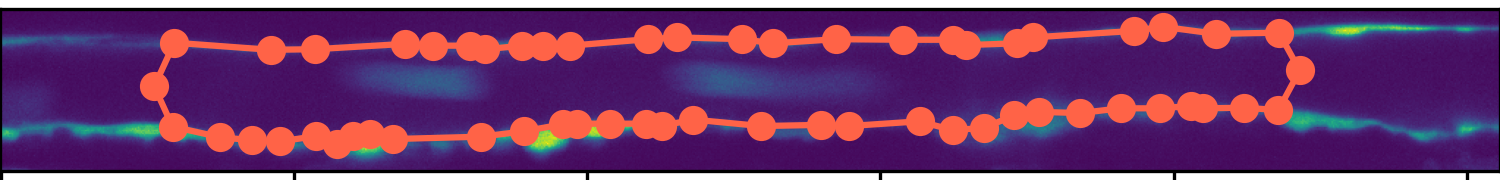
\includegraphics[width=\linewidth]{figures/outline_before_clip.png} \\
    (1)
    \end{subfigure}
    \begin{subfigure}{0.8 \linewidth}
    \centering
    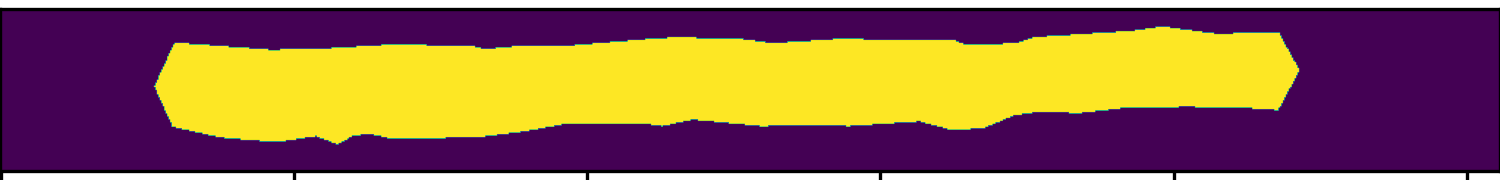
\includegraphics[width=\linewidth]{figures/Polygon_mask.png} \\
    (2)
    \end{subfigure}
    \begin{subfigure}{0.8 \linewidth}
    \centering
    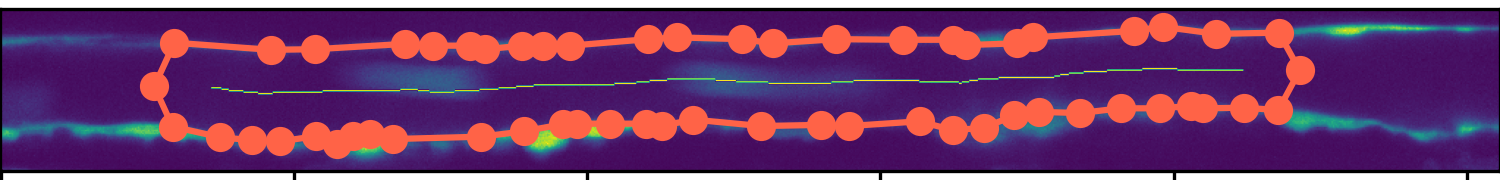
\includegraphics[width=\linewidth]{figures/skeleton_with_outline.png} \\
    (3)
    \end{subfigure}
    
    \begin{subfigure}{0.8 \linewidth}
    \centering
    \begin{subfigure}{0.3 \linewidth}
    \centering
    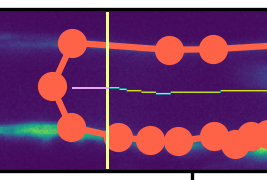
\includegraphics[width=\linewidth]{figures/clipping_full_poly.png}
    (4-a)
    \end{subfigure}
    \begin{subfigure}{0.3 \linewidth}
    \centering
    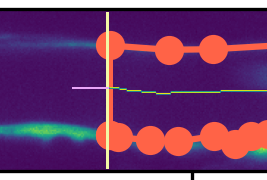
\includegraphics[width=\linewidth]{figures/clipping_clipped_poly.png}
    (4-b)
    \end{subfigure}
    \end{subfigure}
    \begin{subfigure}{0.8 \linewidth}
    \centering
    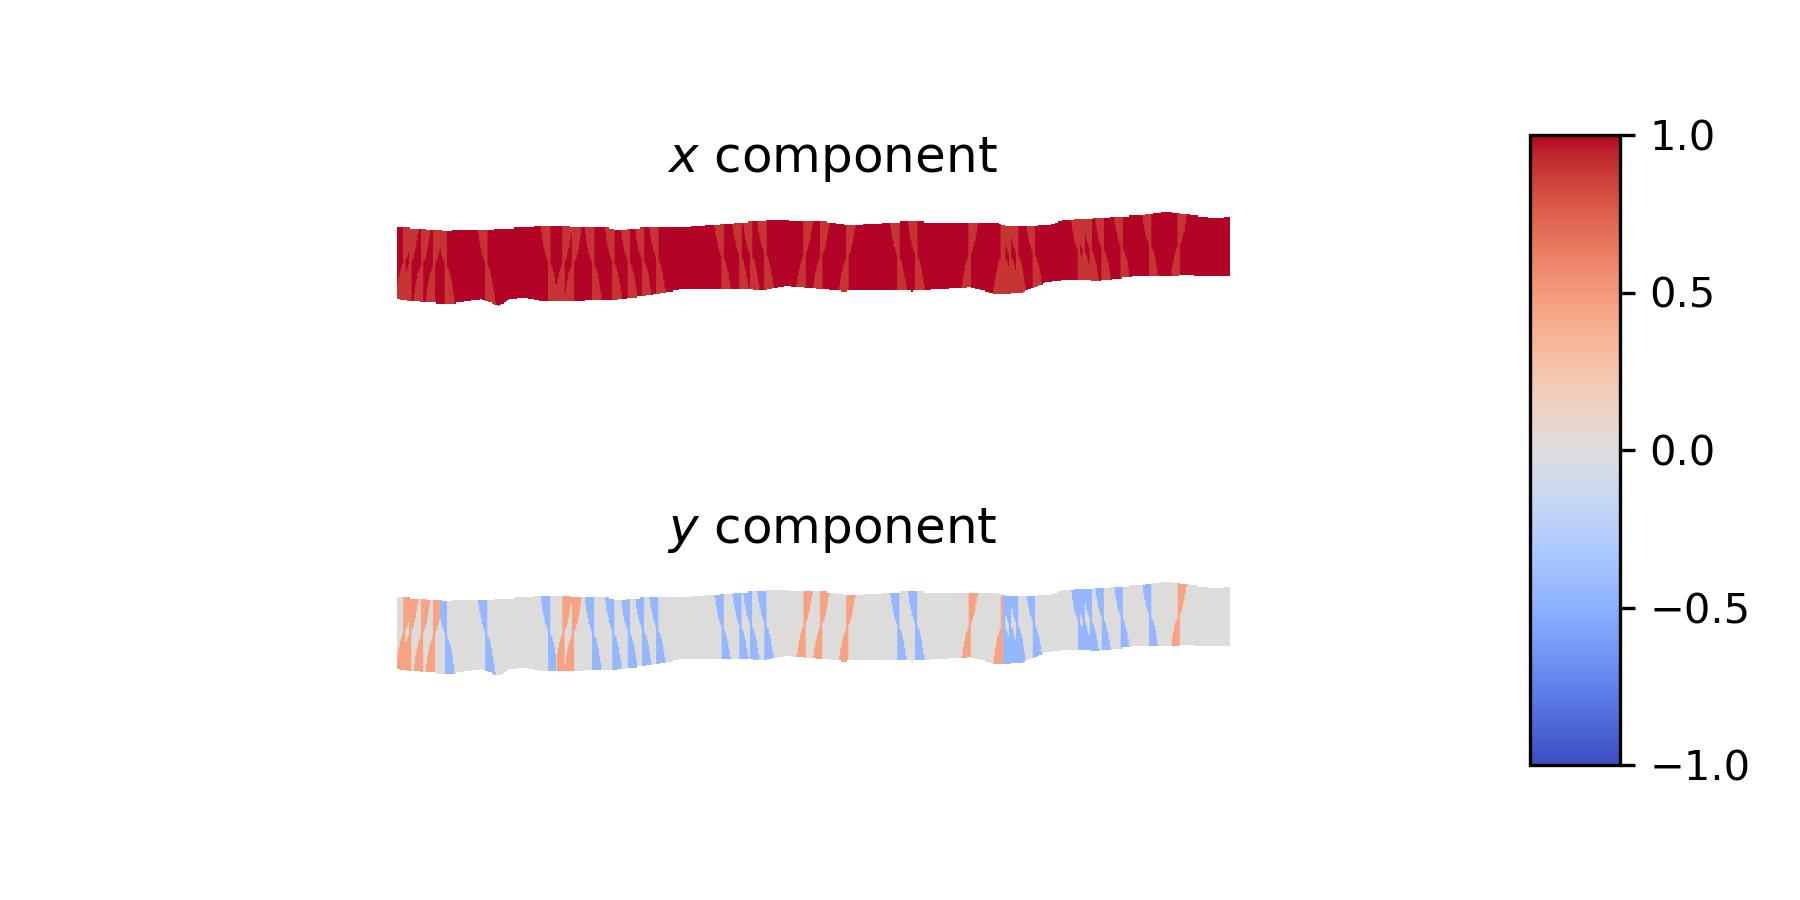
\includegraphics[width=\linewidth]{figures/centerline_direction.png} \\
    (5)
    \end{subfigure}
    
    \caption{From top to bottom: 
    (1) The manually marked ROI, each dot represents a vertex manually added by the user. 
    (2) The polygonal mask generated from the outline.
    (3) The skeleton of the polygonal mask, with the ROI superimposed.
    (4-a) The polygonal mask before clipping, in pink, the estimated direction, in yellow, the centerline normal, used to clip the ROI.
    (4-b) The polygonal mask after clipping, in pink, the estimated direction, in yellow, the centerline normal, used to clip the ROI.
    (5) The directional components of the nearest centerline pixel.}
    \label{fig:roi}
\end{figure}

\subsection{Estimating centerline-distances, and vessel radius}
To estimate the distance to the centerline, we transform the skeletonised ROI with the euclidean distance transform and (bi-)linearly interpolate subpixel differences in the particle positions. To estimate the radius of the blood vessel, we use the maximum distance to the centerline for all particles within the ROI.

\section{Estimating velocities}
To estimate the velocities, we need three things

\begin{enumerate}
    \item The particle tracks
    \item The spatial pixel-dimensions
    \item The time between each frame
\end{enumerate}

The particle tracks were already estimated with the \texttt{scripts/track\_particles.py}-script. However, that script didn't filter tracks by their length. Here, we filter those tracks further by removing all tracks where the particle was present for less than 5 frames. We also remove all tracks outside the ROI.

To compute the spatial pixel-dimensions and the time between each frame, we use the image metadata, obtained with the \texttt{confocal\_microscopy.files.ims.load\_ims\_metadata}-function. We then use the following code to get the image size, pixel size, and timestep. The output of this code is compared with many of the \texttt{legend.docx} files provided by Federico, and these numbers always coincided.

\begin{verbatim}
    ## Get the image metadata
    image_size = ims.find_physical_image_size(metadata)[1:]
    image_shape = [
        int(metadata["CustomData"]["Height"]),
        int(metadata["CustomData"]["Width"])
    ]
    pixel_size = np.round(np.array(image_size) / image_shape, 3)

    timestamps = [
        datetime.fromisoformat(metadata["TimeInfo"][f"TimePoint{i+1}"])
        for i in range(7000)
    ]
    timestamps = [t - timestamps[0] for t in timestamps]
    timestamps = [(t.seconds + t.microseconds*1e-6) for t in timestamps]
    timestamps = np.linspace(0, timestamps[-1], len(timestamps))

    timestep = timestamps[-1]/len(timestamps)
\end{verbatim}

Based on this, we could transform the particle velocities from pixels per frame to $\upmu \text{m}/\text{s}$.

\subsection{Validating the results}
To validate the results from the particle tracking, we manually tracked in a variety of of fishes and vessels. The automatic velocity estimates were generally satisfying with a high sensitivity\footnote{Also known as recall} (most manually tracked particles were found), and a low-medium positive predictive value\footnote{Also known as precision} (the automatic tracking found approximately twice the number of tracks compared to the manual tracking). Some of the tracks found by the automatic algorithm and not manually were false positives and others were actual particles not found during the manual tracking.

To see the results from the manual tracking, see the \texttt{scripts/Early exploratory analysis.ipynb}.

\section{Estimating pressures}
There are several ways to estimate the pressure. If we first assume that we know the viscosity (more about that later), then we can estimate the pressure by

\begin{enumerate}
    \item Using Poiseuille's law and estimating the pressure for each particle independently, and then computing the average pressure gradient
    \item Assume a velocity profile on the form $v(r) = b r^2 - a$ and compute the pressure gradient analytically
\end{enumerate}

With option one, we estimate the pressure-gradient that drives the motion of the $i$-th particle, $|\nabla p_i|$, with the following formula

\begin{equation}
    |\nabla p_i| = 3 v_i \mu / (R - r_i),
\end{equation}

where $v_i$ and $r_i$ is the velocity and distance to centerline for the $i$-th particle, $R$ is the radius of the vessel and $\mu$ is the blood viscosity. To compute the total pressure gradient, $|\nabla p|$, we compute the average of $|\nabla p_i|$.

If we instead assume a monomial+intercept velocity profile, then we estimate the total pressure gradient, $|\nabla p|$, by

\begin{equation}
    |\nabla p| = 4 a \mu / R^2,
\end{equation}

where $a$ is the amplitude of the velocity profile. To estimate the parameters of the velocity profile, we use the fact that $v(R) = 0$ to remove one degree of freedom (the $b$ in $v(r) = b r^2 + a$). Then, we use Brent's root-finding method \cite{brent1973algorithms,virtanen2020scipy} to estimate the $a$ that minimise the squared error $\sum_i (v(r_i) - v_i)^2$.

To estimate the velocities and pressures for a single blood vessels, run the \texttt{scripts/Summary analysis.ipynb}-notebook. To compute for all blood vessels, run the \texttt{scripts/compute\_summaries.py} function.

\subsection{Estimating the viscosity}
There are two ways to estimate the viscosity, either with the method of Lee et al. \cite{lee2017rapid}, who measured the viscosity as a function of tube hematocrit ($ht$) (fraction red blood cells in the blood) in a rectangular channel of size $60\upmu \text{m} \times 240 \upmu \text{m}$. They found that the blood was Newtonian in so large channels, and fitted a quadratic model to the viscosity for $0 \leq ht \lessapprox 0.35$. Moreover, Lee et al. found that zebrafish blood plasma ($ht=0$) has approximately 1.5 the viscosity of water.

The other way of estimating the viscosity of zebrafish blood is with the method of Pries et al. \cite{pries1992blood}, who combined many estimates of human blood viscosity and found that the viscosity varies greatly with the vessel radius and discharge hematocrit (fraction of red blood cells in blood that is released through an open blood vessel). They fitted a complicated heuristic model based on a variety of properties of human blood. One of which was that human blood plasma has the same viscosity as water. This model is therefore not fully compatible with the findings of \cite{lee2017rapid}.

To conclude, we see that there is no accurate measurement of zebrafish blood viscosity. The measurements by Lee et al. does not account for small vessels, where the red blood cells interact with the vessel walls, whereas the model by Pries et al. is based on human blood, which has different properties compared to the blood of zebrafish.

\printbibliography

\end{document}
